\begin{center}
    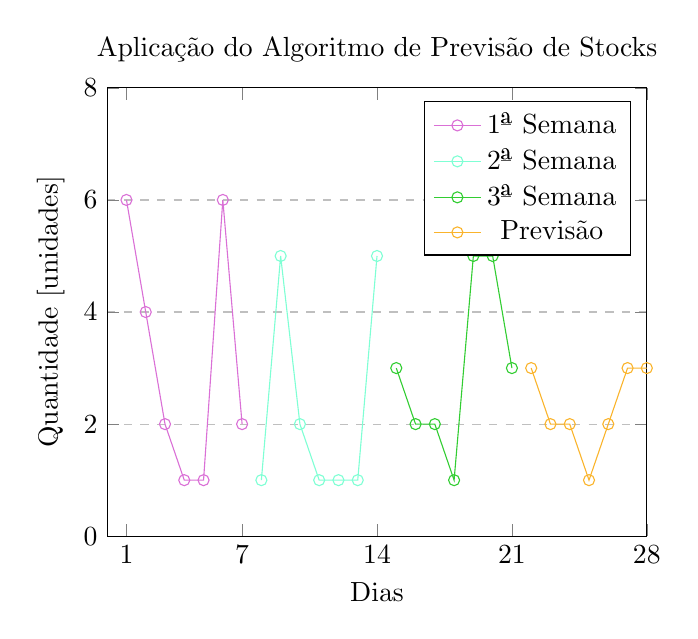
\begin{tikzpicture}
        \begin{axis}[
            title={Aplicação do Algoritmo de Previsão de Stocks},
            xlabel={Dias},
            ylabel={Quantidade [unidades]},
            xmin=0, xmax=28,
            ymin=0, ymax=8,
            xtick={1, 7, 14, 21, 28},
            ytick={},
            legend pos=north east,
            ymajorgrids=true,
            grid style=dashed,
        ]
        \addplot[
            color=Orchid,
            mark=o,
            ]
            coordinates {
            (1,6)(2,4)(3,2)(4,1)(5,1)(6,6)(7,2)
            };
            
        \addplot[
            color=Aquamarine,
            mark=o,
            ]
            coordinates {
            (8,1)(9,5)(10,2)(11,1)(12,1)(13,1)(14,5)
            };
            
        \addplot[
            color=LimeGreen,
            mark=o,
            ]
            coordinates {
            (15,3)(16,2)(17,2)(18,1)(19,5)(20,5)(21,3)
            };
            
        \addplot[
            color=Dandelion,
            mark=o,
            ]
            coordinates {
            (22,3)(23,2)(24,2)(25,1)(26,2)(27,3)(28,3)
            };
            
            \legend{1ª Semana,2ª Semana,3ª Semana,Previsão}
            
        \end{axis}
    \end{tikzpicture}
\end{center}



